%%%%%%%%%%%%%%%%%%%%%%% 子系统及其接口设计 %%%%%%%%%%%%%%%%%%%%%%%%%%%%%%%%%%%%%%%%%%%%%
\chapter{子系统及其接口设计}

\section{确定设计类}
    在用例析取和类的合并的基础上,我们得出”鲜天下“平台由三个子系统构成:订单系统、用户系统和钱包系统;这三个系统通过订单控制类或用户控制类分别对主订单实体或用户实体进行操作。其中的每个系统、控制类和实体都可以作为一个设计类来编写代码。所以平台的设计类图如下\autoref{fig:design_class}。

    \begin{figure}[htp]
        %\begin{adjustwidth}{-1.5cm}{-1cm}
        \centering
        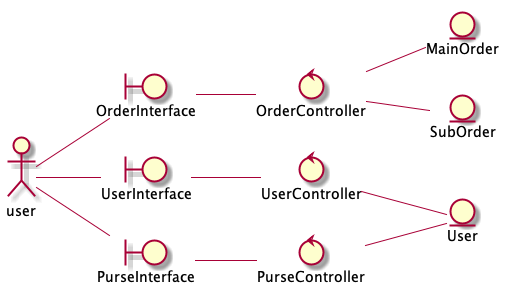
\includegraphics[width=12cm]{report/figure/subsystem/design_class.png}
        \caption{“鲜天下”平台设计类图}
        \label{fig:design_class}
        %\end{adjustwidth}
    \end{figure}

\section{定义子系统}
    我们在上述的分析基础上,可以看出“鲜天下”平台由订单系统(OrderSystem)、用户系统(UserSystem)和钱包系统(PurseSystem)构成,三者的示意图分别如\autoref{fig:OrderSystem}、\autoref{fig:UserSystem}、\autoref{fig:PurseSystem}所示。

    \begin{figure}[htp]
        %\begin{adjustwidth}{-1.5cm}{-1cm}
        \centering
        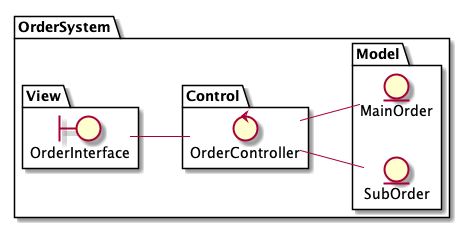
\includegraphics[width=12cm]{report/figure/subsystem/OrderSystem.png}
        \caption{“鲜天下”平台订单子系统架构图}
        \label{fig:OrderSystem}
        %\end{adjustwidth}
    \end{figure}
    
    \begin{figure}[htp]
        %\begin{adjustwidth}{-1.5cm}{-1cm}
        \centering
        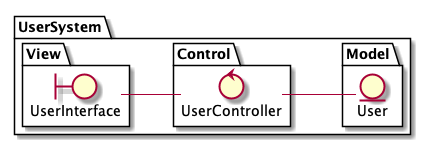
\includegraphics[width=12cm]{report/figure/subsystem/UserSystem.png}
        \caption{“鲜天下”平台用户子系统架构图}
        \label{fig:UserSystem}
        %\end{adjustwidth}
    \end{figure}
    
    \begin{figure}[htp]
        %\begin{adjustwidth}{-1.5cm}{-1cm}
        \centering
        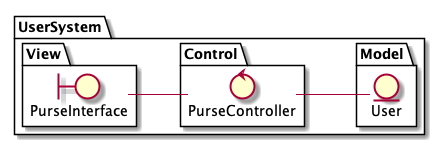
\includegraphics[width=12cm]{report/figure/subsystem/PurseSystem.png}
        \caption{“鲜天下”平台钱包子系统架构图}
        \label{fig:PurseSystem}
        %\end{adjustwidth}
    \end{figure}

\section{定义接口}
    在上述架构图中,View层给出了子系统的接口,订单子系统接口如图\autoref{fig:OrderInterface}所示。
    \begin{figure}[htp]
        %\begin{adjustwidth}{-1.5cm}{-1cm}
        \centering
        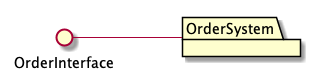
\includegraphics[width=12cm]{report/figure/subsystem/OrderInterface.png}
        \caption{“鲜天下”平台订单子系统接口示意图}
        \label{fig:OrderInterface}
        %\end{adjustwidth}
    \end{figure}
    
    用户子系统接口如图\autoref{fig:UserInterface}所示。
    \begin{figure}[htp]
        %\begin{adjustwidth}{-1.5cm}{-1cm}
        \centering
        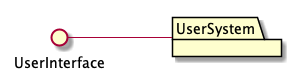
\includegraphics[width=12cm]{report/figure/subsystem/UserInterface.png}
        \caption{“鲜天下”平台用户子系统接口示意图}
        \label{fig:UserInterface}
        %\end{adjustwidth}
    \end{figure}
    
    钱包子系统接口如图\autoref{fig:PurseInterface}所示。
    \begin{figure}[htp]
        %\begin{adjustwidth}{-1.5cm}{-1cm}
        \centering
        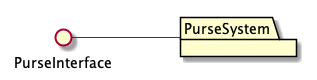
\includegraphics[width=12cm]{report/figure/subsystem/PurseInterface.png}
        \caption{“鲜天下”平台钱包子系统接口示意图}
        \label{fig:PurseInterface}
        %\end{adjustwidth}
    \end{figure}
    
\section{确定可重用子系统}
    在本次项目中,订单系统(OrderSystem)、用户系统(UserSystem)和钱包系统(PurseSystem)均可重用或嵌入到其他的系统设计中。